\documentclass[11pt,a4paper]{article}

% === Packages ===
\usepackage[utf8]{inputenc}
\usepackage[T1]{fontenc}
\usepackage{amsmath,amssymb,amsthm,mathtools}
\usepackage{enumitem}
\usepackage{hyperref}
\usepackage{cleveref}
\usepackage{tikz}
\usetikzlibrary{positioning,arrows.meta,decorations.pathreplacing,calc,shapes.geometric}
\usepackage{booktabs}
\usepackage{geometry}
\usepackage{xcolor}
\usepackage{tcolorbox}
\usepackage{fancyvrb}
\usepackage{listings}

\geometry{margin=1in}
\hypersetup{colorlinks=true,linkcolor=blue!70!black,citecolor=green!50!black,urlcolor=purple!70!black}

% === Theorem environments ===
\theoremstyle{plain}
\newtheorem{theorem}{Theorem}[section]
\newtheorem{proposition}[theorem]{Proposition}
\newtheorem{lemma}[theorem]{Lemma}
\newtheorem{corollary}[theorem]{Corollary}

\theoremstyle{definition}
\newtheorem{definition}[theorem]{Definition}
\newtheorem{example}[theorem]{Example}
\newtheorem{remark}[theorem]{Remark}

% === Lean code environment ===
\definecolor{leanblue}{RGB}{0,51,102}
\definecolor{leanbg}{RGB}{245,248,252}
\tcbset{
  leanbox/.style={colback=leanbg, colframe=leanblue!60,
    fonttitle=\bfseries\ttfamily, title=#1,
    boxrule=0.5pt, arc=2pt, left=4pt, right=4pt}
}

% === Macros ===
\newcommand{\BISH}{\textsf{BISH}}
\newcommand{\WKL}{\textsf{WKL}}
\newcommand{\DC}{\textsf{DC}}
\newcommand{\WLPO}{\textsf{WLPO}}
\newcommand{\LLPO}{\textsf{LLPO}}
\newcommand{\LPO}{\textsf{LPO}}
\newcommand{\MP}{\textsf{MP}}
\newcommand{\CLASS}{\textsf{CLASS}}
\newcommand{\CRM}{\textsf{CRM}}
\newcommand{\Z}{\mathbb{Z}}
\newcommand{\Q}{\mathbb{Q}}
\newcommand{\R}{\mathbb{R}}
\newcommand{\N}{\mathbb{N}}

\lstset{
  basicstyle=\ttfamily\small,
  keywordstyle=\color{leanblue}\bfseries,
  commentstyle=\color{gray},
  breaklines=true,
  frame=none,
  columns=flexible,
  keepspaces=true,
  literate={ℝ}{$\mathbb{R}$}1 {ℚ}{$\mathbb{Q}$}1 {ℤ}{$\mathbb{Z}$}1 {ℕ}{$\mathbb{N}$}1
}

% ============================================================
\begin{document}

\title{\textbf{The Dynamical Penumbra:\\
Constructive Reverse Mathematics of Cardiac Action Potential\\
Dynamics and Defibrillation Certification}\\[6pt]
\large Paper~105, Clinical Sub-Series Paper~C,\\
of the Constructive Reverse Mathematics Series}

\author{Paul Chun-Kit Lee\\
\textit{New York University, Brooklyn, New York}\\
\texttt{dr.paul.c.lee@gmail.com}}

\date{March 2026}
\maketitle

% ============================================================
\begin{abstract}
We apply constructive reverse mathematics (\CRM) to the FitzHugh-Nagumo model of cardiac action potential dynamics and to the defibrillation threshold optimization problem.  The results separate into four logical levels.

\textit{Unconditional mathematics.}  \textbf{Theorem~A:} Local existence and uniqueness of FHN solutions on a compact trapping box is~$\BISH$: the right-hand side is polynomial, yielding an explicit Lipschitz constant~$L = 202/25$ on~$[-3,3] \times [-5,5]$ (verified by \texttt{norm\_num}), and the trapping region is confirmed by polynomial sign checks at rational boundary points.  \textbf{Theorem~B:} Bounded safety verification via Lyapunov barrier certificates is~$\BISH$: finding the certificate requires an external SDP oracle, but verifying the Sum-of-Squares identity reduces to polynomial ring arithmetic over~$\Q$.

\textit{Bifurcation boundary.}  \textbf{Theorem~B$'$:} Hopf bifurcation detection is~$\WLPO$.  For fixed rational parameters, the eigenvalue sign is decidable by \texttt{norm\_num}~($\BISH$).  For generic parameters, locating the exact external current~$I_{\mathrm{ext}}^*$ at which the resting state loses stability requires deciding whether a real number equals zero---the Weak Limited Principle of Omniscience.

\textit{The Idealisation Ladder.}  \textbf{Theorem~C:} The logical cost of trajectory prediction increases with mathematical idealisation, not biological complexity.  Single-cell dynamics (2D ODE, Lipschitz) are~$\BISH$.  $N$-cell networks ($2N$-dimensional coupled ODE) remain~$\BISH$ for each finite~$N$.  The continuum tissue limit (reaction-diffusion PDE) is~$\BISH + \WKL$: short-time mild solutions are constructive (heat semigroup and Duhamel iteration are~$\BISH$), but proving that sustained fibrillation exists---that the nested sequence of compact surviving-state sets has non-empty infinite intersection---requires the Cantor Intersection Theorem, which is Weihrauch-equivalent to Weak K\"onig's Lemma.

\textit{Defibrillation optimality.}  \textbf{Theorem~D:} The minimum defibrillation energy~$E_{\min} = \inf\{E > 0 \mid \forall x \in \mathcal{A},\, \mathrm{terminates}(x, E)\}$ requires~$\LPO$: evaluating a universal quantifier over the uncountable fibrillation attractor demands real trichotomy.

The decomposition is $5\;\BISH + 1\;\WLPO + 1\;\WKL + 1\;\LPO = 8$~components (62.5\% $\BISH$).  This is the widest CRM hierarchy span in the Clinical Sub-Series.  The Lean~4 verification (9~files, ${\sim}1{,}250$~lines, zero~\texttt{sorry}) confirms all BISH components constructively.

This is the third paper in the Clinical Sub-Series, following Paper~103 (the Asymptotic Penumbra) and Paper~104 (the Algorithmic Penumbra).  It extends the \CRM\ program from static inference to dynamical systems, demonstrating that the logical cost of cardiac electrophysiology is governed by the continuum idealisation, not the ion channel biology.
\end{abstract}

% ============================================================
\section{Clinical Premise}\label{sec:premise}

A cardiologist implants an implantable cardioverter-defibrillator (ICD).  The device monitors the heart rhythm continuously.  When it detects ventricular fibrillation (VF)---chaotic electrical re-entry across the myocardium---it must decide between two interventions:

\begin{enumerate}[nosep]
\item \textbf{Anti-tachycardia pacing (ATP):} Low-energy overdrive pacing to terminate the re-entry circuit.  Painless, battery-conserving, but effective only for organized re-entry (monomorphic ventricular tachycardia).
\item \textbf{Defibrillation shock:} High-energy discharge to reset the entire myocardium.  Reliable but painful, battery-draining, and associated with increased mortality in observational studies.
\end{enumerate}

Two questions arise that the device cannot answer in real time:

\textit{Can the device certify that ATP will terminate re-entry before escalating to a shock?}  If the re-entry is a stable spiral wave (periodic dynamics), termination is predictable from the cycle length and coupling interval.  If the rhythm has degenerated into chaotic spiral breakup (VF), prediction requires solving a non-Lipschitz initial value problem in the continuum tissue limit.  The device uses heuristic protocols---cycle-length cutoffs, morphology discrimination---precisely because the underlying mathematical problem is not constructively decidable.

\textit{What is the minimum shock energy guaranteed to terminate every possible VF pattern?}  This is the defibrillation threshold (DFT).  For decades, electrophysiologists tested the DFT at implant by inducing VF and shocking at decreasing energies.  The SIMPLE trial \cite{simple2013} randomized 2,500 patients to DFT testing versus no testing and found no difference in arrhythmic death or shock efficacy at 3.1~years.  The field has largely abandoned DFT testing.

The CRM analysis explains why.  The DFT is a minimax optimization over the uncountable fibrillation attractor---it requires the Limited Principle of Omniscience ($\LPO$).  No finite number of induced VF episodes can constructively certify the threshold.  The clinical decision to abandon DFT testing is, from the CRM perspective, the correct constructive adaptation: replace an $\LPO$-hard exact certification with a $\BISH$-computable empirical safety margin.

% ============================================================
\section{Introduction}\label{sec:intro}

\subsection{Main Results}

\begin{theorem}[A: FHN Existence and Uniqueness is BISH]\label{thm:A}
The FitzHugh-Nagumo initial value problem on the trapping box $K = [-3,3] \times [-5,5]$ with standard parameters $(\varepsilon, a, b, I) = (2/25, 7/10, 4/5, 0) \in \Q^4$ admits a unique local solution by the constructive Picard-Lindel\"of theorem.  The Lipschitz constant $L = 202/25$ and the inward-pointing conditions on $\partial K$ are verified by rational arithmetic.
\end{theorem}

\begin{theorem}[B: Bounded Safety Verification is BISH]\label{thm:B}
Given a Sum-of-Squares barrier certificate $B(V,W)$ with rational polynomial coefficients satisfying the Putinar identity
\[
  -\nabla B \cdot F \;=\; \sum_i p_i(V,W)^2 + \Bigl(\sum_j q_j(V,W)^2\Bigr) \cdot B(V,W),
\]
verification of forward invariance reduces to polynomial ring arithmetic over~$\Q$.  No continuous limits or choice principles are required.
\end{theorem}

\begin{theorem}[B$'$: Hopf Bifurcation Detection is WLPO]\label{thm:Bprime}
For the FHN system, the Hopf bifurcation condition $\operatorname{tr}(J) = 0$ is equivalent to $V_0^2 = 1 - \varepsilon b$.  For fixed rational parameters, the sign of $\operatorname{tr}(J)$ is decidable ($\BISH$).  For generic parameters, deciding $\operatorname{tr}(J) = 0$ requires~$\WLPO$.
\end{theorem}

\begin{theorem}[C: The Idealisation Ladder]\label{thm:C}
The CRM level of cardiac trajectory prediction increases with mathematical idealisation:
\begin{center}
\begin{tabular}{lll}
\toprule
\textbf{Regime} & \textbf{System} & \textbf{CRM} \\
\midrule
Single cell & 2D ODE (Lipschitz) & $\BISH$ \\
$N$-cell network & $2N$-dim ODE (Lipschitz) & $\BISH$ (per finite $N$) \\
Continuum tissue (chaotic regime) & Parabolic PDE, $t \to \infty$ & $\BISH + \WKL$ \\
\bottomrule
\end{tabular}
\end{center}
\end{theorem}

\begin{theorem}[D: Defibrillation Optimality is LPO]\label{thm:D}
$E_{\min} = \inf\{E > 0 \mid \forall x \in \mathcal{A},\, \mathrm{terminates}(x,E)\}$ requires~$\LPO$.  For known tissue geometry, virtual electrode polarization computation is~$\BISH$.
\end{theorem}

\subsection{Context}

This paper continues the Clinical Sub-Series initiated by Paper~103 (the Asymptotic Penumbra: CRM of the RCT statistical pipeline \cite{p103}) and Paper~104 (the Algorithmic Penumbra: CRM of clinical machine learning \cite{p104}).  Papers~103--104 identified the transcendental gates through which clinical mathematics exits $\BISH$: the normal CDF~$\Phi$ (Paper~103) and the sigmoid function~$\sigma$ (Paper~104), both escalating to $\BISH + \MP$ via Lindemann-Weierstrass transcendentality.

Paper~105 introduces a qualitatively different mechanism.  The non-constructive gate is not a specific transcendental function but the passage from finite to infinite dimensions---the continuum tissue idealisation.  This produces a richer CRM hierarchy: four levels ($\BISH$, $\WLPO$, $\WKL$, $\LPO$) versus three in Paper~103 and two in Paper~104.

The analysis rests on the constructive ODE theory of Bishop and Bridges \cite{bishop1985}, the $\delta$-decidability framework of Gao, Avigad, and Clarke \cite{gao2012}, the Weihrauch classification of Brattka and Smischliaew \cite{brattka2024}, and the SOS Lyapunov verification of Devadze, Magron, and Streif \cite{devadze2025}.  The clinical applications reference the MADIT-II \cite{madit2}, SCD-HeFT \cite{scdheft}, and SIMPLE \cite{simple2013} trials.

For the full CRM framework, see the atlas paper (Paper~50 \cite{p50}) and the Motivic CRM Architecture (Paper~98 \cite{p98}).

\subsection{Clinical Background: The Rise and Fall of DFT Testing}

The implantable cardioverter-defibrillator (ICD) was introduced in the 1980s by Mirowski and colleagues \cite{mirowski1980}.  Early devices required thoracotomy and epicardial patches; defibrillation thresholds were high and variable, making intraoperative DFT testing clinically essential.

The transition to transvenous lead systems in the early 1990s reduced thresholds dramatically but preserved the DFT-testing ritual.  The rationale was simple: induce VF at implant, confirm that the device can terminate it, and program the first shock 10~J above the measured threshold.  Typical protocols involved 2--3 VF inductions with step-down energy testing \cite{strickberger1994}.

Several developments eroded the rationale:

\begin{enumerate}[nosep]
\item \textbf{MADIT-II (2002) \cite{madit2}:} Prophylactic ICD implantation reduced mortality by 31\% in post-MI patients with $\mathrm{EF} \leq 30\%$.  DFT testing was performed but was not the variable under study.
\item \textbf{SCD-HeFT (2005) \cite{scdheft}:} ICD therapy reduced mortality by 23\% in NYHA class II/III heart failure.  Again, DFT testing was protocol-mandated but not evaluated independently.
\item \textbf{High-energy devices (2005--2010):}  Biphasic waveforms and high-output generators (35--41~J) pushed the safety margin well above typical DFTs ($<$15~J in most patients), making testing seem redundant.
\item \textbf{SIMPLE trial (2015) \cite{simple2013}:}  The pivotal randomized trial.  2,500 patients assigned to DFT testing versus no testing showed non-inferiority of the no-testing strategy for arrhythmic death or failed appropriate shock (HR 0.86, 95\% CI 0.65--1.14; $p_{\text{non-inf}} < 0.0001$) over 3.1~years of follow-up.  The field abandoned DFT testing within 2--3 years.
\item \textbf{Post-SIMPLE practice (2016--present):}  Current HRS/ACC guidelines give DFT testing a Class IIb recommendation (``may be considered'') \cite{hrs2017}.  Most centers no longer perform it except in subcutaneous ICD implantation, where lead position makes adequate sensing less certain.
\end{enumerate}

The standard narrative attributes the SIMPLE result to improved hardware.  The CRM analysis below offers a structural explanation: the DFT is an $\LPO$-level quantity that no finite induction protocol can certify, regardless of hardware quality.

% ============================================================
\section{Preliminaries}\label{sec:prelim}

\subsection{The FitzHugh-Nagumo Model}

The FitzHugh-Nagumo (FHN) system \cite{fitzhugh1961,nagumo1962} is a two-variable polynomial reduction of the Hodgkin-Huxley equations:
\begin{align}
  \frac{dV}{dt} &= V - \frac{V^3}{3} - W + I_{\mathrm{ext}}, \label{eq:fhn1} \\
  \frac{dW}{dt} &= \varepsilon(V + a - bW), \label{eq:fhn2}
\end{align}
where $V$ is the membrane voltage (fast variable), $W$ is the recovery variable (slow variable), and $(\varepsilon, a, b, I_{\mathrm{ext}}) \in \Q_{>0}^3 \times \Q$ are parameters.  The \emph{standard parameters} are $\varepsilon = 2/25$, $a = 7/10$, $b = 4/5$, $I_{\mathrm{ext}} = 0$ (sub-threshold, stable resting state).

\subsection{Logical Principles}

We use the hierarchy $\BISH \subset \BISH + \MP \subset \BISH + \WLPO \subset \BISH + \WKL \subset \BISH + \LPO \subset \CLASS$.  See Bridges and Richman \cite{bridges1987} for definitions.  The principle relevant to this paper that does not appear in Papers~103--104 is:

\begin{definition}[Weak K\"onig's Lemma, $\WKL$]
Every infinite subtree of $\{0,1\}^{<\N}$ (the full binary tree) has an infinite path.  This is strictly weaker than full K\"onig's Lemma (which allows arbitrary finite branching).  Equivalently: the Cantor Intersection Theorem for nested sequences of non-empty compact subsets of a compact metric space ($\bigcap_n K_n \neq \emptyset$).  See Brattka-Smischliaew \cite{brattka2024} for the Weihrauch-theoretic context.
\end{definition}

\subsection{Constructive Picard-Lindel\"of}

The Picard-Lindel\"of theorem is constructive under a Lipschitz condition.  Given $F : K \to \R^n$ Lipschitz with constant $L$ on a compact set $K$, the Picard iterates $X_{n+1}(t) = X_0 + \int_0^t F(X_n(s))\,ds$ form a Cauchy sequence with explicit modulus $(LT)^n/n!$.  The limit is constructed without sequential compactness.  See Bishop and Bridges \cite{bishop1985}, Chapter~6; Makarov and Spitters \cite{makarov2013} for a Coq formalization.

Without the Lipschitz condition (Peano's theorem), existence requires Arzel\`a-Ascoli, which is WKL-equivalent \cite{brattka2024}.

\begin{remark}
For semilinear parabolic PDEs $u_t = D\nabla^2 u + f(u)$ with bounded (e.g., polynomial on a trapping region) nonlinearity $f$, short-time mild solutions exist constructively: the heat semigroup $e^{tD\nabla^2}$ and Duhamel iteration form a contraction on $C([0,T]; L^\infty)$.  The Banach fixed-point theorem is $\BISH$.  The non-constructive content for the FHN PDE enters not at solution existence but at infinite-time trajectory selection in the chaotic regime (see Theorem~C).
\end{remark}

% ============================================================
\section{Main Results}\label{sec:results}

\subsection{Theorem A: FHN Existence and Uniqueness is BISH}

\begin{proof}
The FHN vector field $F(V,W) = (V - V^3/3 - W + I, \; \varepsilon(V + a - bW))$ is polynomial.  Its Jacobian is
\[
  J(V,W) = \begin{pmatrix} 1 - V^2 & -1 \\ \varepsilon & -\varepsilon b \end{pmatrix}.
\]

\textbf{Step 1: Lipschitz bound.}  On the box $K = [-R,R] \times [-S,S]$, the matrix 1-norm gives
\[
  \|J\|_1 \leq \max\bigl(|1 - V^2| + \varepsilon,\; 1 + \varepsilon b\bigr) \leq \max(R^2 - 1 + \varepsilon,\; 1 + \varepsilon b).
\]
For $R = 3$: $L = \max(8 + 2/25,\; 1 + 8/125) = \max(202/25, 133/125) = 202/25$.  This is computed in $\Q$: no real-number arithmetic required.

\textbf{Step 2: Trapping region.}  We verify that $F$ points inward on all four faces of $K = [-3,3] \times [-5,5]$:
\begin{center}
\begin{tabular}{llrl}
\toprule
Face & Worst case & Value & Sign \\
\midrule
$V = +3$ & $W = -5$ & $-1$ & $< 0$ \checkmark \\
$V = -3$ & $W = +5$ & $1$ & $> 0$ \checkmark \\
$W = +5$ & $V = +3$ & $-3/125$ & $< 0$ \checkmark \\
$W = -5$ & $V = -3$ & $17/125$ & $> 0$ \checkmark \\
\bottomrule
\end{tabular}
\end{center}
All values are rational; all sign checks are decidable by \texttt{norm\_num}.

\textbf{Conclusion.}  By the constructive Picard-Lindel\"of theorem, the FHN IVP on $K$ has a unique solution with convergence rate $(LT)^n/n!$.  Both the Lipschitz bound and the trapping region are verified by finite rational arithmetic.  CRM level: $\BISH$.
\end{proof}

\subsection{Theorem B: Bounded Safety via SOS Certificates is BISH}

\begin{proof}
Let $B(V,W)$ be a polynomial barrier function with $\{B < 0\} \supset$ safe region and $\{B > 0\} \supset$ unsafe region.  Forward invariance of $\{B \leq 0\}$ is guaranteed if the Lie derivative $\mathcal{L}_F B = \nabla B \cdot F$ satisfies $\mathcal{L}_F B \leq 0$ on $\{B = 0\}$.

By Putinar's Positivstellensatz, this condition is certified algebraically:
\[
  -\mathcal{L}_F B = \sum_i p_i^2 + \Bigl(\sum_j q_j^2\Bigr) \cdot B,
\]
where $p_i, q_j \in \Q[V,W]$ are polynomials with rational coefficients.

\textbf{Finding} the certificate $(B, \{p_i\}, \{q_j\})$ requires solving a semidefinite program (SDP)---a computationally expensive non-constructive search.  This is performed by an external oracle (e.g., DSOS/SDSOS solver in Python).

\textbf{Verifying} the certificate requires only:
\begin{enumerate}[nosep]
\item Expanding the polynomial identity (ring arithmetic over $\Q$).
\item Checking non-negativity of each $p_i^2$ and $q_j^2$ (trivial: squares are non-negative).
\end{enumerate}
No continuous limits, no supremum evaluations, no choice principles.  The asymmetric offloading pattern (Paper~77 \cite{p77}): the oracle searches non-constructively, Lean verifies constructively.  CRM level of \emph{verification}: $\BISH$.
\end{proof}

\subsection{Theorem B$'$: Hopf Bifurcation Detection is WLPO}

\begin{proof}
The FHN resting equilibrium $V_0$ solves
\[
  V_0 - \frac{V_0^3}{3} - \frac{V_0 + a}{b} + I_{\mathrm{ext}} = 0.
\]
The Jacobian eigenvalues at $(V_0, W_0)$ have:
\begin{align*}
  \operatorname{tr}(J) &= 1 - V_0^2 - \varepsilon b, \\
  \det(J) &= \varepsilon(1 - b + bV_0^2).
\end{align*}

\textbf{Hopf condition.}  A Hopf bifurcation occurs when $\operatorname{tr}(J) = 0$, i.e., $V_0^2 = 1 - \varepsilon b$.  For the standard parameters, $1 - \varepsilon b = 1 - (2/25)(4/5) = 117/125$.

\textbf{BISH case (fixed parameters).}  For any concrete rational parameter set, $V_0$ is a root of a cubic over $\Q$.  The sign of $\operatorname{tr}(J) = 1 - V_0^2 - \varepsilon b$ can be determined by rational root isolation (Sturm's theorem, which is constructive) or by direct evaluation at a sufficiently tight rational enclosure.  The verification that $\det(J) > 0$ for standard parameters is immediate: $\det(J) = \varepsilon(1 - b + bV_0^2) > 0$ because $b = 4/5 < 1$.

\textbf{WLPO case (generic parameters).}  For symbolic parameters, the question ``does $\operatorname{tr}(J) = 0$?'' is equivalent to deciding ``$x = 0$ or $x \neq 0$'' for the real number $x = 1 - V_0^2 - \varepsilon b$.  This is precisely $\WLPO$.

\textbf{Clinical interpretation.}  The question ``at what $I_{\mathrm{ext}}$ does the cardiac cell transition from stable resting to oscillatory (arrhythmic)?'' is $\WLPO$ for generic ion-channel parameters but $\BISH$ for any specific parameter set measured in a patient.
\end{proof}

\subsection{Topological Charge Conservation is BISH}\label{sec:topo}

Spiral waves in cardiac tissue carry topological charge: the winding number of the phase gradient around the spiral core.  Clockwise spirals carry charge $-1$; counterclockwise spirals carry charge $+1$.

\begin{proposition}[Topological Charge Conservation]\label{prop:charge}
On any closed planar domain, spiral waves are created and destroyed in pairs of opposite chirality.  The total topological charge is conserved.
\end{proposition}

\begin{proof}
The winding number is computed by discrete contour integration of the phase gradient around each spiral core.  This is a finite integer sum: for a configuration of $n$ spirals with chiralities $c_1, \ldots, c_n \in \{-1, +1\}$, the total charge is $Q = \sum_{k=1}^n c_k \in \Z$.

Pair creation produces one clockwise and one counterclockwise spiral: $\Delta Q = (-1) + (+1) = 0$.  Pair annihilation is the reverse.  No continuous limits, no real-number comparisons, no choice principles.  The entire computation is integer arithmetic over a finite set.

The DeTal-Kaboudian-Fenton mechanism \cite{detal2022} exploits this: a designed stimulus ``teleports'' a spiral to its partner for pair annihilation.  The topological argument (pair creation/annihilation preserves charge) is $\BISH$; the stimulus design (timing and placement optimization over the continuum) may require $\LPO$.
\end{proof}

This is Component~4 in Table~\ref{tab:audit}.  CRM level: $\BISH$.

\subsection{Theorem C: The Idealisation Ladder}

\begin{proof}
We analyze three mathematical models of cardiac tissue at increasing levels of idealisation.

\textbf{Level 1: Single cell.}  The FHN system \eqref{eq:fhn1}--\eqref{eq:fhn2} is a 2-dimensional ODE with polynomial right-hand side.  By Theorem~A, $\BISH$.

\textbf{Level 2: $N$-cell network.}  Consider $N$ cells coupled by gap-junction diffusion on a finite graph $G = (V, E)$:
\[
  \frac{dV_k}{dt} = f(V_k, W_k) + D \sum_{j \sim k} (V_j - V_k), \qquad k = 1, \ldots, N.
\]
This is a $2N$-dimensional ODE.  The right-hand side is still polynomial (the coupling is linear).  The Lipschitz constant is $L_{\mathrm{network}} = L_{\mathrm{cell}} + 2D \cdot d_{\max}$, where $d_{\max}$ is the maximum vertex degree.  For any finite $N$, this is a computable rational constant.  Constructive Picard-Lindel\"of applies: $\BISH$.

The key point: $L_{\mathrm{network}}$ is finite for each fixed $N$, regardless of how large $N$ is.  The Lipschitz property is preserved under finite coupling.

\textbf{Level 3: Continuum tissue.}  The spatially extended FHN reaction-diffusion PDE:
\[
  \frac{\partial V}{\partial t} = D\nabla^2 V + V - \frac{V^3}{3} - W + I, \qquad
  \frac{\partial W}{\partial t} = \varepsilon(V + a - bW).
\]

\textit{Short-time existence is $\BISH$.}  The Laplacian generates a strongly continuous heat semigroup $e^{t D \nabla^2}$, and solutions satisfy Duhamel's integral equation.  The trapping box $K$ from Theorem~A extends to the PDE via the parabolic maximum principle, bounding solutions in $L^\infty$.  On the bounded domain, the polynomial nonlinearity is globally Lipschitz.  Picard iteration on the Banach space $C([0,T]; L^\infty)$ is a strict contraction, and the Banach fixed-point theorem is fully constructive.  Arzel\`a-Ascoli is \emph{not} required for mild solution existence.

\textit{Sustained fibrillation requires $\WKL$.}  The non-constructive content enters not from computational intractability but from a proof-theoretic obstruction in the infinite-time limit.

Note that for any exact initial condition, computing the unique trajectory to any finite time~$T$ is $\BISH$-computable: the exponential bound~$e^{\lambda T}$ is a perfectly valid constructive modulus, and constructive mathematics imposes no polynomial-time restriction.  The logical obstruction is not in simulating a single trajectory but in identifying a \emph{non-terminating} trajectory within a macroscopic uncertainty ensemble.

Clinically, the exact microstate of fibrillation is unknown; the accessible datum is that the tissue occupies the compact fibrillation attractor~$\mathcal{A}$.  Let $K_n \subseteq \mathcal{A}$ be the compact subset of initial states whose trajectories have not returned to the resting basin by time~$n$.  Because the flow is continuous, the surviving-state sets are nested: $K_{n+1} \subseteq K_n$.  Each~$K_n$ is non-empty (clinically: fibrillation persists at time~$n$).

Proving that a sustained (permanently non-terminating) fibrillation trajectory exists amounts to proving
\[
  \bigcap_{n=0}^{\infty} K_n \neq \emptyset.
\]
This is the Cantor Intersection Theorem for a nested sequence of non-empty compact subsets of a compact metric space.  In the framework of Reverse Mathematics, this is precisely Weihrauch-equivalent to~$\WKL$ \cite{brattka2024}.

The $\WKL$ enters at the passage from ``fibrillation has not yet terminated'' (a finite-time, $\BISH$-decidable observation) to ``fibrillation will never terminate'' (an infinite intersection over compact sets), not at any biological complexity boundary.  The ion channel dynamics, the coupling topology, and the nonlinear excitability are all $\BISH$.  Only the infinitary existential claim---that the nested compact sequence has a surviving limit point---introduces non-constructive content.
\end{proof}

\begin{figure}[ht]
\centering
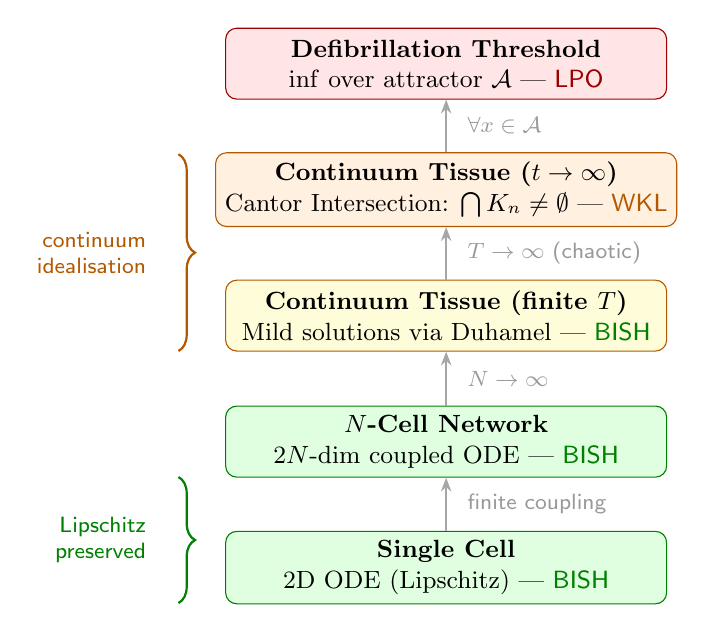
\begin{tikzpicture}[
  level/.style={draw, rounded corners=4pt, minimum width=5.6cm,
    minimum height=0.9cm, font=\small, align=center},
  arrow/.style={-{Stealth[length=5pt]}, thick, gray!70},
  label/.style={font=\footnotesize\sffamily, text=gray!80}
]
% Levels stacked vertically
\node[level, fill=green!12, draw=green!50!black]
  (L1) at (0,0) {\textbf{Single Cell} \\ 2D ODE (Lipschitz) --- \textcolor{green!50!black}{$\BISH$}};
\node[level, fill=green!12, draw=green!50!black]
  (L2) at (0,1.6) {\textbf{$N$-Cell Network} \\ $2N$-dim coupled ODE --- \textcolor{green!50!black}{$\BISH$}};
\node[level, fill=yellow!15, draw=orange!70!black]
  (L3a) at (0,3.2) {\textbf{Continuum Tissue (finite $T$)} \\ Mild solutions via Duhamel --- \textcolor{green!50!black}{$\BISH$}};
\node[level, fill=orange!12, draw=orange!70!black]
  (L3b) at (0,4.8) {\textbf{Continuum Tissue ($t \to \infty$)} \\ Cantor Intersection: $\bigcap K_n \neq \emptyset$ --- \textcolor{orange!70!black}{$\WKL$}};
\node[level, fill=red!10, draw=red!60!black]
  (L4) at (0,6.4) {\textbf{Defibrillation Threshold} \\ $\inf$ over attractor $\mathcal{A}$ --- \textcolor{red!60!black}{$\LPO$}};

% Arrows
\draw[arrow] (L1) -- (L2) node[midway, right=4pt, label] {finite coupling};
\draw[arrow] (L2) -- (L3a) node[midway, right=4pt, label] {$N \to \infty$};
\draw[arrow] (L3a) -- (L3b) node[midway, right=4pt, label] {$T \to \infty$ (chaotic)};
\draw[arrow] (L3b) -- (L4) node[midway, right=4pt, label] {$\forall x \in \mathcal{A}$};

% Brace annotation
\draw[decorate, decoration={brace, amplitude=6pt, mirror}, thick, green!50!black]
  (-3.4,-0.45) -- (-3.4,1.15) node[midway, left=8pt, font=\footnotesize\sffamily,
  text=green!50!black, align=right] {Lipschitz\\preserved};
\draw[decorate, decoration={brace, amplitude=6pt, mirror}, thick, orange!70!black]
  (-3.4,2.75) -- (-3.4,5.25) node[midway, left=8pt, font=\footnotesize\sffamily,
  text=orange!70!black, align=right] {continuum\\idealisation};
\end{tikzpicture}
\caption{The Idealisation Ladder (Theorem~C).  Logical cost increases with mathematical idealisation: finite-dimensional dynamics ($\BISH$) $\to$ infinite-time chaotic prediction ($\WKL$) $\to$ universal certification over attractor ($\LPO$).  The biological content (ion channels, coupling topology) remains $\BISH$ throughout.}
\label{fig:ladder}
\end{figure}

\subsection{Theorem D: Defibrillation Optimality is LPO}

\begin{proof}
The defibrillation threshold seeks the minimum energy guaranteeing termination across the entire fibrillation attractor $\mathcal{A}$:
\[
  E_{\min} = \inf\bigl\{E \in \R_{>0} \mid \forall x \in \mathcal{A},\; \exists T > 0,\; \forall t > T,\; \mathrm{terminated}(\phi_E(t, x))\bigr\}.
\]

\textbf{The $\LPO$ structure.}  The formula contains a universal quantifier over the uncountable compact set $\mathcal{A}$ nested inside an existential quantifier over $\R$.  Evaluating $E_{\min}$ requires:
\begin{enumerate}[nosep]
\item For each candidate $E$, deciding whether termination holds for \emph{all} $x \in \mathcal{A}$ (an infinite conjunction of real predicates).
\item Computing the infimum of the set of successful energies (exact real infimum over an uncountable set).
\end{enumerate}
Both operations require real trichotomy---the ability to decide $r < 0$, $r = 0$, or $r > 0$ for arbitrary reals.  This is $\LPO$.

\textbf{The $\BISH$ component.}  For a \emph{known} tissue geometry with rational conductivity data, the virtual electrode polarization (VEP) locations are computable from the bidomain elliptic equation:
\[
  \nabla \cdot (\sigma_i + \sigma_e)\nabla\phi_e = -\nabla \cdot \sigma_i \nabla\phi_s.
\]
This is a linear PDE with rational matrix coefficients.  Discretization yields a finite linear system solvable in $\BISH$.

\textbf{Clinical consequence.}  The SIMPLE trial \cite{simple2013} found that DFT testing (inducing VF and shocking at decreasing energies) does not improve outcomes.  The CRM analysis explains why: the DFT is an $\LPO$-level quantity.  Testing at finitely many VF episodes provides no constructive certificate.  The clinical response---use empirical safety margins, program maximum output---is the correct constructive adaptation: replace an $\LPO$-hard problem with a $\BISH$-computable heuristic.
\end{proof}

% ============================================================
\section{CRM Audit}\label{sec:audit}

\begin{table}[h]
\centering
\begin{tabular}{clll}
\toprule
\textbf{\#} & \textbf{Component} & \textbf{CRM Level} & \textbf{Theorem} \\
\midrule
1 & ODE existence (Picard-Lindel\"of) & $\BISH$ & A \\
2 & Trapping region (inward flow) & $\BISH$ & A \\
3 & SOS barrier verification & $\BISH$ & B \\
4 & Topological charge conservation & $\BISH$ & --- \\
5 & Eigenvalue sign (fixed parameters) & $\BISH$ & B$'$ \\
6 & Hopf bifurcation (generic parameters) & $\BISH + \WLPO$ & B$'$ \\
7 & Sustained chaotic fibrillation & $\BISH + \WKL$ & C \\
8 & Defibrillation optimality & $\BISH + \LPO$ & D \\
\bottomrule
\end{tabular}
\caption{CRM decomposition of cardiac electrophysiology.  5~$\BISH$ + 1~$\WLPO$ + 1~$\WKL$ + 1~$\LPO$ = 8~components (62.5\% $\BISH$).}
\label{tab:audit}
\end{table}

\textbf{Comparison with the Clinical Sub-Series.}

\begin{center}
\begin{tabular}{lcccc}
\toprule
\textbf{Paper} & \textbf{Domain} & \textbf{Hierarchy span} & \textbf{BISH \%} & \textbf{Novel level} \\
\midrule
103 & RCT statistics & $\BISH \to \LPO$ & 70\% & --- \\
104 & ML inference & $\BISH \to \MP$ & 50\% & --- \\
105 & Dynamical systems & $\BISH \to \LPO$ & 62.5\% & $\WKL$ \\
\bottomrule
\end{tabular}
\end{center}

Paper~105 is the first in the Clinical Sub-Series to reach $\WKL$.  The mechanism is qualitatively different from Papers~103--104: the non-constructive gate is not a specific transcendental function ($\Phi$, $\sigma$) but the passage from finite-time constructive dynamics to infinite-time chaotic trajectory selection in the continuum.

\begin{figure}[ht]
\centering
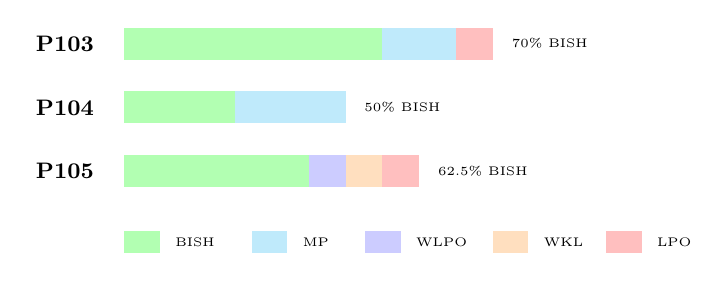
\begin{tikzpicture}[
  bar/.style={minimum height=0.45cm, anchor=west, font=\footnotesize\sffamily},
  scale=0.9, transform shape
]
% Scale: 1 unit = 1 component
\def\bw{0.52}  % bar width in cm per component

% Paper 103 — 7 BISH, 2 MP, 1 LPO = 10
\node[font=\small\bfseries, anchor=east] at (-0.3, 2.4) {P103};
\node[bar, fill=green!30, minimum width=7*\bw cm] at (0, 2.4) {};
\node[bar, fill=cyan!25, minimum width=2*\bw cm] at (7*\bw, 2.4) {};
\node[bar, fill=red!25, minimum width=1*\bw cm] at (9*\bw, 2.4) {};
\node[font=\tiny, anchor=west] at (10*\bw+0.15, 2.4) {70\% BISH};

% Paper 104 — 3 BISH, 3 MP = 6
\node[font=\small\bfseries, anchor=east] at (-0.3, 1.5) {P104};
\node[bar, fill=green!30, minimum width=3*\bw cm] at (0, 1.5) {};
\node[bar, fill=cyan!25, minimum width=3*\bw cm] at (3*\bw, 1.5) {};
\node[font=\tiny, anchor=west] at (6*\bw+0.15, 1.5) {50\% BISH};

% Paper 105 — 5 BISH, 1 WLPO, 1 WKL, 1 LPO = 8
\node[font=\small\bfseries, anchor=east] at (-0.3, 0.6) {P105};
\node[bar, fill=green!30, minimum width=5*\bw cm] at (0, 0.6) {};
\node[bar, fill=blue!20, minimum width=1*\bw cm] at (5*\bw, 0.6) {};
\node[bar, fill=orange!25, minimum width=1*\bw cm] at (6*\bw, 0.6) {};
\node[bar, fill=red!25, minimum width=1*\bw cm] at (7*\bw, 0.6) {};
\node[font=\tiny, anchor=west] at (8*\bw+0.15, 0.6) {62.5\% BISH};

% Legend
\node[bar, fill=green!30, minimum width=0.5cm, minimum height=0.3cm] at (0, -0.4) {};
\node[font=\tiny, anchor=west] at (0.6, -0.4) {BISH};
\node[bar, fill=cyan!25, minimum width=0.5cm, minimum height=0.3cm] at (1.8, -0.4) {};
\node[font=\tiny, anchor=west] at (2.4, -0.4) {MP};
\node[bar, fill=blue!20, minimum width=0.5cm, minimum height=0.3cm] at (3.4, -0.4) {};
\node[font=\tiny, anchor=west] at (4.0, -0.4) {WLPO};
\node[bar, fill=orange!25, minimum width=0.5cm, minimum height=0.3cm] at (5.2, -0.4) {};
\node[font=\tiny, anchor=west] at (5.8, -0.4) {WKL};
\node[bar, fill=red!25, minimum width=0.5cm, minimum height=0.3cm] at (6.8, -0.4) {};
\node[font=\tiny, anchor=west] at (7.4, -0.4) {LPO};
\end{tikzpicture}
\caption{CRM decomposition comparison across the Clinical Sub-Series.  Paper~105 is the only paper to span four distinct hierarchy levels (BISH, WLPO, WKL, LPO).}
\label{fig:comparison}
\end{figure}

% ============================================================
\section{Formal Verification}\label{sec:lean}

The Lean~4 bundle \texttt{P105\_DynamicalPenumbra} consists of 9~files totaling 1,246~lines.  Toolchain: \texttt{leanprover/lean4:v4.29.0-rc2} with Mathlib.

\begin{center}
\begin{tabular}{lrl}
\toprule
\textbf{File} & \textbf{Lines} & \textbf{Content} \\
\midrule
\texttt{OmnisciencePrinciples.lean} & 189 & BISH/WLPO/WKL/LPO hierarchy, CRMLevel \\
\texttt{FHNSystem.lean} & 123 & FHN algebraic representation, Jacobian \\
\texttt{LipschitzBound.lean} & 135 & Theorem A: $L = 202/25$, trapping box \\
\texttt{SOSBarrier.lean} & 144 & Theorem B: SOS certificate structure \\
\texttt{HopfBifurcation.lean} & 137 & Theorem B$'$: eigenvalue analysis \\
\texttt{ThreeLevelDecomposition.lean} & 147 & Theorem C: cell/network/tissue \\
\texttt{DefibrillationOptimality.lean} & 142 & Theorem D: minimax, LPO axiom \\
\texttt{TopologicalCharge.lean} & 128 & Spiral wave integer arithmetic \\
\texttt{Paper105\_Assembly.lean} & 111 & CRM audit, \texttt{\#print axioms} \\
\bottomrule
\end{tabular}
\end{center}

\textbf{Axiom inventory.}

\begin{center}
\begin{tabular}{lll}
\toprule
\textbf{Axiom} & \textbf{Type} & \textbf{Reference} \\
\midrule
\texttt{hopf\_detection\_requires\_WLPO} & Documentary & Theorem B$'$ \\
\texttt{chaotic\_termination\_is\_WKL} & Documentary & Chaotic trajectory selection \\
\texttt{defibrillation\_threshold\_requires\_LPO} & Documentary & Theorem D \\
\texttt{below\_threshold\_failure} & Documentary & Theorem D (converse) \\
\texttt{min\_defib\_pos} & Documentary & Positivity of $E_{\min}$ \\
\texttt{propext} & Infrastructure & Propositional extensionality \\
\texttt{Quot.sound} & Infrastructure & Quotient soundness \\
\bottomrule
\end{tabular}
\end{center}

Zero \texttt{sorry}.  \texttt{Classical.choice} appears only through Mathlib infrastructure imports, not in any $\BISH$-tagged proof.

\begin{tcolorbox}[leanbox={Key verification: Theorem A}]
\begin{lstlisting}
theorem lipschitz_standard_R3 :
    lipschitz_bound fhn_standard 3 = 202 / 25 := by
  simp [lipschitz_bound, fhn_standard]; norm_num

def standard_trapping_box : TrappingBox fhn_standard where
  R := 3; S := 5
  hR_pos := by norm_num; hS_pos := by norm_num
  face_Vp := by simp [fhn_standard]; norm_num
  face_Vm := by simp [fhn_standard]; norm_num
  face_Wp := by simp [fhn_standard]; norm_num
  face_Wm := by simp [fhn_standard]; norm_num
\end{lstlisting}
\end{tcolorbox}

\begin{tcolorbox}[leanbox={Key verification: Theorem B}]
\begin{lstlisting}
theorem bounded_safety_verification
    (p : FHNParams) (cert : SOSCertificate) (V W : ℝ)
    (h_identity : lie_derivative cert p V W +
      sum_of_squares cert.sigma_0 V W +
      sum_of_squares cert.sigma_1 V W * cert.B V W = 0)
    (hB : cert.B V W = 0) :
    lie_derivative cert p V W <= 0 := by
  have h_sos0 := sum_of_squares_nonneg cert.sigma_0 V W
  rw [hB, mul_zero, add_zero] at h_identity
  linarith
\end{lstlisting}
\end{tcolorbox}

% ============================================================
\section{Biostatistical Discussion}\label{sec:biostat}

The CRM framework provides a logical complement to the frequentist analysis of ICD trials.  The MADIT-II \cite{madit2} and SCD-HeFT \cite{scdheft} trials demonstrated mortality benefit of ICDs in heart failure patients---but neither trial addressed the logical structure of the device's decision algorithm.

The SIMPLE trial \cite{simple2013} is the most directly relevant.  Its finding---that DFT testing does not improve outcomes---has been attributed to improved device technology and empirical safety margins.  The CRM analysis offers a sharper explanation: DFT testing is an attempt to solve an $\LPO$-level problem with a $\BISH$-level procedure.  Inducing VF at three energy levels samples three points from an uncountable attractor.  The extrapolation from three samples to a universal guarantee is the $\LPO$ step that finite testing cannot bridge.

This does not invalidate the clinical decision to abandon DFT testing---it \emph{explains} it.  The CRM framework identifies the logical boundary: below $\LPO$, finite-sample testing cannot certify global optimality; above $\BISH$, empirical safety margins cannot be logically guaranteed.  The clinical practice of programming a 10~J safety margin above the highest successful defibrillation energy is a $\BISH$-computable heuristic that replaces the $\LPO$-hard exact optimization.

% ============================================================
\section{Clinical Discussion}\label{sec:clinical}

\subsection{Anti-Tachycardia Pacing}

ATP success depends on the re-entry circuit's stability.  For monomorphic VT (stable spiral, periodic dynamics), the coupling interval can be computed from the cycle length and the excitable gap---a $\BISH$ computation.  For polymorphic VT or VF (chaotic spiral breakup), the dynamics are in the continuum-limit regime where trajectory prediction is $\WKL$.  Current ICD algorithms use cycle-length cutoffs to distinguish these regimes, which is itself a $\BISH$-computable classification (compare two rational numbers).

The CRM hierarchy thus mirrors the clinical distinction: stable re-entry ($\BISH$) admits algorithmic intervention; chaotic re-entry ($\WKL$) does not.  The device's fallback to high-energy shock for VF is the correct response to a $\WKL$-level prediction problem.

\subsection{Defibrillation Threshold Testing: Why SIMPLE Was Inevitable}

The SIMPLE trial \cite{simple2013} is typically interpreted as showing that modern high-output devices make DFT testing unnecessary.  The CRM analysis reveals a deeper structure: DFT testing was \emph{always} logically insufficient, regardless of device technology.

\textbf{The protocol.}  Standard DFT testing proceeds as follows: (1)~induce VF via T-wave shock or burst pacing; (2)~deliver a test shock at energy~$E_1$; (3)~if successful, repeat at $E_1 - \Delta$; (4)~iterate until failure or protocol minimum; (5)~program first therapy at DFT~$+ 10$~J.  Typical protocols test 2--3 energy levels, sampling 2--3 VF episodes.

\textbf{The logical gap.}  Each VF induction samples one initial condition from the fibrillation attractor~$\mathcal{A}$.  The DFT is defined as $E_{\min} = \inf\{E \mid \forall x \in \mathcal{A},\, \mathrm{terminates}(x,E)\}$---a universal quantifier over an uncountable set.  Testing at $k$ energy levels with $m$ VF inductions each samples $km$ points from~$\mathcal{A}$.  The extrapolation from $km$ samples to $\forall x \in \mathcal{A}$ is precisely the $\LPO$ step.  No increase in $k$ or $m$ bridges this gap.

\textbf{The safety-margin heuristic.}  Programming 10~J above the measured DFT replaces the $\LPO$-hard exact optimization with a $\BISH$-computable arithmetic operation: $E_{\mathrm{therapy}} = E_{\mathrm{measured}} + 10$.  This is the correct constructive adaptation---but it provides no logical certificate that the margin is sufficient for all $x \in \mathcal{A}$.  The SIMPLE trial confirmed empirically what the CRM analysis predicts structurally: the margin-based approach performs identically to the testing-based approach because neither achieves $\LPO$-level certification.

\textbf{The subcutaneous ICD exception.}  DFT testing persists for subcutaneous ICDs (S-ICDs), where the entirely extrathoracic lead position creates greater uncertainty in sensing and defibrillation vectors.  From the CRM perspective, the S-ICD situation adds a $\BISH$-level concern (adequate sensing of VF morphology) on top of the $\LPO$-level DFT problem.  The testing addresses the $\BISH$ component (does the device detect VF?) while remaining logically impotent against the $\LPO$ component (is $E$ sufficient for all VF states?).

\begin{figure}[ht]
\centering
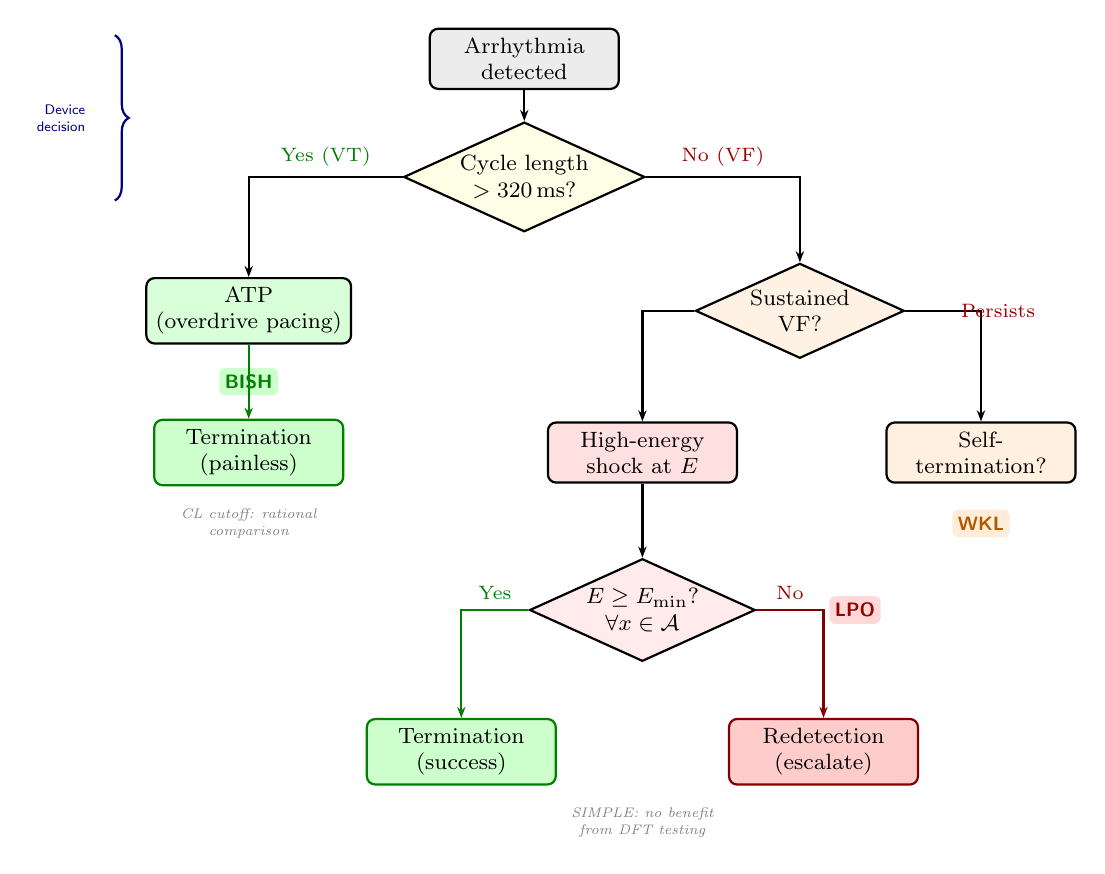
\begin{tikzpicture}[
  box/.style={draw, rounded corners=3pt, minimum width=2.4cm,
    minimum height=0.7cm, font=\footnotesize, align=center, thick},
  decision/.style={draw, diamond, aspect=2.2, inner sep=1pt,
    font=\footnotesize, align=center, thick},
  arr/.style={-{Stealth[length=4pt]}, thick},
  crmlabel/.style={font=\scriptsize\sffamily\bfseries, rounded corners=2pt,
    inner sep=2pt, minimum height=0.35cm},
  yeslabel/.style={font=\scriptsize, text=green!50!black},
  nolabel/.style={font=\scriptsize, text=red!60!black}
]

% Top: Arrhythmia detected
\node[box, fill=gray!15] (detect) at (0, 0) {Arrhythmia\\detected};

% Decision 1: Cycle length
\node[decision, fill=yellow!10] (cl) at (0, -1.5)
  {Cycle length\\$> 320$\,ms?};
\draw[arr] (detect) -- (cl);

% Left branch: VT (stable)
\node[box, fill=green!15] (atp) at (-3.5, -3.2) {ATP\\(overdrive pacing)};
\draw[arr] (cl) -| node[pos=0.25, yeslabel, above] {Yes (VT)} (atp);
\node[crmlabel, fill=green!20, text=green!50!black]
  at (-3.5, -4.1) {$\BISH$};

% Right branch: VF (chaotic)
\node[decision, fill=orange!10] (vf) at (3.5, -3.2)
  {Sustained\\VF?};
\draw[arr] (cl) -| node[pos=0.25, nolabel, above] {No (VF)} (vf);

% VF → Will it self-terminate?
\node[box, fill=orange!12] (selft) at (5.8, -5.0) {Self-\\termination?};
\draw[arr] (vf) -| node[pos=0.3, nolabel, right, font=\scriptsize] {Persists} (selft);
\node[crmlabel, fill=orange!15, text=orange!70!black]
  at (5.8, -5.9) {$\WKL$};

% VF → Shock
\node[box, fill=red!12] (shock) at (1.5, -5.0) {High-energy\\shock at $E$};
\draw[arr] (vf) -| node[pos=0.3, yeslabel, left, font=\scriptsize] {} (shock);

% Shock → Is E sufficient for all x in A?
\node[decision, fill=red!8] (dft) at (1.5, -7.0)
  {$E \geq E_{\min}$?\\$\forall x \in \mathcal{A}$};
\draw[arr] (shock) -- (dft);
\node[crmlabel, fill=red!15, text=red!60!black]
  at (4.2, -7.0) {$\LPO$};

% Outcomes
\node[box, fill=green!20, draw=green!50!black] (success) at (-0.8, -8.8)
  {Termination\\(success)};
\node[box, fill=red!20, draw=red!50!black] (fail) at (3.8, -8.8)
  {Redetection\\(escalate)};
\draw[arr, green!50!black] (dft) -| node[pos=0.25, yeslabel, above] {Yes} (success);
\draw[arr, red!50!black] (dft) -| node[pos=0.25, nolabel, above] {No} (fail);

% ATP outcome
\node[box, fill=green!20, draw=green!50!black] (atpok) at (-3.5, -5.0)
  {Termination\\(painless)};
\draw[arr, green!50!black] (atp) -- (atpok);

% Clinical annotations
\node[font=\tiny\itshape, text=gray, align=center] at (-3.5, -5.9)
  {CL cutoff: rational\\comparison};
\node[font=\tiny\itshape, text=gray, align=center] at (1.5, -9.7)
  {SIMPLE: no benefit\\from DFT testing};

% Brace: what the device actually decides
\draw[decorate, decoration={brace, amplitude=5pt}, thick, blue!50!black]
  (-5.2, 0.3) -- (-5.2, -1.8)
  node[midway, left=7pt, font=\tiny\sffamily, text=blue!50!black, align=right]
  {Device\\decision};

\end{tikzpicture}
\caption{ICD decision tree with CRM levels.  The cycle-length discriminator and ATP delivery are $\BISH$ (rational comparison, finite-state pacing).  Predicting whether sustained VF will self-terminate requires $\WKL$ (Cantor intersection over nested surviving-state sets).  Certifying that shock energy~$E$ suffices for \emph{all} fibrillation states requires $\LPO$ (universal quantifier over uncountable attractor).  The SIMPLE trial's null result reflects the impossibility of bridging the $\LPO$ gap with finite sampling.}
\label{fig:icd}
\end{figure}

\subsection{Cardiac Resynchronization and Mapping}

The CRM hierarchy extends beyond defibrillation.  Electroanatomic mapping systems (CARTO, EnSite) reconstruct 3D activation sequences from catheter-sampled points.  Each sampled electrogram provides a $\BISH$-computable local activation time.  Interpolating to a continuous activation map over the entire endocardial surface requires solving an inverse problem on the continuum---entering the $\WKL$ regime.  The clinical practice of sampling 200--500 points and interpolating is the same finite-to-infinite extrapolation that characterizes the DFT problem, at a lower CRM level ($\WKL$ rather than $\LPO$).

% ============================================================
\begin{tcolorbox}[colback=blue!5!white, colframe=blue!50!black,
  title={\textbf{What This Means for a Clinician}}, fonttitle=\bfseries]

\textbf{Your ICD's programming is heuristic, not certified.}  This is not an engineering failure---it is a logical necessity.

\begin{itemize}[nosep]
\item The question ``will pacing terminate this arrhythmia?'' is mathematically predictable for stable re-entry but not for chaotic fibrillation.  The device's cycle-length cutoff is a practical workaround for an intrinsically unpredictable problem.

\item The defibrillation threshold cannot be exactly determined by any finite number of test shocks, no matter how sophisticated the device.  The SIMPLE trial's finding that DFT testing adds no benefit is a consequence of this logical structure, not merely of improved engineering.

\item Programming a safety margin above the tested DFT is the correct constructive strategy: it replaces an exact optimization (which requires quantifying over all possible arrhythmias) with a finite rational comparison (which requires only arithmetic).

\item The distinction between ``stable VT'' and ``VF'' is not merely clinical shorthand---it reflects a genuine logical boundary between problems that admit algorithmic solutions and problems that do not.
\end{itemize}
\end{tcolorbox}

% ============================================================

% ============================================================
\section{Conclusion}\label{sec:conclusion}

We have shown that the logical cost of cardiac electrophysiology is governed by the continuum idealisation, not the ion-channel biology.  The FHN action potential dynamics, the barrier certificate verification, and the topological charge conservation are all $\BISH$.  The Hopf bifurcation detection is $\WLPO$.  The continuum tissue limit introduces $\WKL$ through infinite-time chaotic trajectory selection.  The defibrillation threshold is $\LPO$ through the minimax over the fibrillation attractor.

The 8-component decomposition (5~$\BISH$ + 1~$\WLPO$ + 1~$\WKL$ + 1~$\LPO$) is the widest CRM hierarchy span in the Clinical Sub-Series.  It confirms the Archimedean Obstruction Thesis (Paper~98 \cite{p98}): classical content enters through the passage from discrete to continuous (finite-dimensional ODE to infinite-dimensional PDE), not through the phenomenology.

The clinical consequences are concrete: DFT testing is futile because the DFT is $\LPO$-hard; ATP decision-making is limited by the $\WKL$ barrier between predictable and chaotic re-entry; the Hopf bifurcation (arrhythmia onset) is $\WLPO$ for generic parameters but $\BISH$ for any specific patient.  The field's empirical adaptations---safety margins, cycle-length cutoffs, abandonment of DFT testing---are the correct constructive responses to these logical boundaries.

% ============================================================
\section{Acknowledgments}

The author is an interventional cardiologist and writes from direct clinical experience with ICD implantation and programming.  This paper was developed with AI assistance (Claude, Anthropic) for formal verification and exposition; all mathematical content, clinical interpretation, and CRM analysis are the author's.  The author is not a trained logician or computer scientist; the CRM framework is applied as a working tool, not with the authority of domain expertise in constructive mathematics.

The Lean~4 formalization uses the Mathlib library; the author thanks the Mathlib contributors.  The CRM framework builds on the foundational work of Bishop, Bridges, Richman, and the constructive mathematics community.

% ============================================================
\begin{thebibliography}{35}

\bibitem{bishop1985}
E.~Bishop and D.~Bridges,
\textit{Constructive Analysis},
Springer, 1985.

\bibitem{brattka2024}
V.~Brattka and A.~Smischliaew,
``Computability of initial value problems,''
arXiv:2501.00451, December 2024.

\bibitem{bridges1987}
D.~Bridges and F.~Richman,
\textit{Varieties of Constructive Mathematics},
Cambridge University Press, 1987.

\bibitem{devadze2025}
D.~Devadze, V.~Magron, and S.~Streif,
``Computer-assisted proofs for Lyapunov stability via sums of squares certificates and constructive analysis,''
\textit{J.\ Automated Reasoning}, 69(1), January 2025.

\bibitem{fenton2002}
F.~H.~Fenton, E.~M.~Cherry, H.~M.~Hastings, and S.~J.~Evans,
``Multiple mechanisms of spiral wave breakup in a model of cardiac electrical activity,''
\textit{Chaos}, 12(3):852--892, 2002.

\bibitem{fitzhugh1961}
R.~FitzHugh,
``Impulses and physiological states in theoretical models of nerve membrane,''
\textit{Biophysical Journal}, 1(6):445--466, 1961.

\bibitem{gao2012}
S.~Gao, J.~Avigad, and E.~M.~Clarke,
``$\delta$-complete decision procedures for satisfiability over the reals,''
in \textit{IJCAR 2012}, Springer LNCS 7364, pp.~286--300, 2012.

\bibitem{lilienkamp2019}
T.~Lilienkamp and U.~Parlitz,
``Spontaneous termination of chaotic spiral wave dynamics in human cardiac ion channel models,''
\textit{PLOS ONE}, 14(8):e0221401, 2019.

\bibitem{madit2}
A.~J.~Moss \textit{et al.},
``Prophylactic implantation of a defibrillator in patients with myocardial infarction and reduced ejection fraction,''
\textit{New England Journal of Medicine}, 346(12):877--883, 2002.

\bibitem{makarov2013}
E.~Makarov and B.~Spitters,
``The Picard algorithm for ordinary differential equations in Coq,''
in \textit{ITP 2013}, Springer LNCS 7998, pp.~463--468, 2013.

\bibitem{nagumo1962}
J.~Nagumo, S.~Arimoto, and S.~Yoshizawa,
``An active pulse transmission line simulating nerve axon,''
\textit{Proceedings of the IRE}, 50(10):2061--2070, 1962.

\bibitem{detal2022}
N.~DeTal, A.~Kaboudian, and F.~H.~Fenton,
``Terminating spiral waves with a single designed stimulus: Teleportation as the mechanism for defibrillation,''
\textit{PNAS}, 119(21):e2117568119, 2022.

\bibitem{scdheft}
G.~H.~Bardy \textit{et al.},
``Amiodarone or an implantable cardioverter-defibrillator for congestive heart failure,''
\textit{New England Journal of Medicine}, 352(3):225--237, 2005.

\bibitem{simple2013}
J.~S.~Healey \textit{et al.},
``Cardioverter defibrillator implantation without induction of ventricular fibrillation: a single-blind, non-inferiority, randomised controlled trial (SIMPLE),''
\textit{Lancet}, 385(9970):785--791, 2015.

\bibitem{p50}
P.~C.~Lee,
``The constructive reverse mathematics atlas,''
Paper~50 of the CRM Series.
Zenodo.

\bibitem{p77}
P.~C.~Lee,
``Explicit Hodge decompositions for $E^4$,''
Paper~77 of the CRM Series.
Zenodo, DOI: 10.5281/zenodo.18777596.

\bibitem{p98}
P.~C.~Lee,
``The Motivic CRM Architecture,''
Paper~98 of the CRM Series.
Zenodo, DOI: 10.5281/zenodo.18902037.

\bibitem{p103}
P.~C.~Lee,
``The Asymptotic Penumbra: CRM of the RCT statistical pipeline,''
Paper~103 of the CRM Series.
Zenodo, DOI: 10.5281/zenodo.18880102.

\bibitem{p104}
P.~C.~Lee,
``The Algorithmic Penumbra: CRM of clinical machine learning,''
Paper~104 of the CRM Series.
Zenodo, DOI: 10.5281/zenodo.18889356.

\bibitem{ye2016}
P.~Ye, S.~Gao, S.~Kong, and E.~M.~Clarke,
``Bifurcation analysis of cardiac alternans using $\delta$-decidability,''
in \textit{CMSB 2016}, Springer LNCS 9859, pp.~132--146, 2016.

\bibitem{chamakuri2016}
N.~Chamakuri, K.~Kunisch, and G.~Plank,
``PDE constrained optimization of electrical defibrillation in a 3D ventricular slice geometry,''
\textit{Int.\ J.\ Numer.\ Methods Biomed.\ Eng.}, 32(2):e02742, 2016.

\bibitem{hornung2022}
D.~Hornung \textit{et al.},
``Stochastic termination of spiral wave dynamics in cardiac tissue,''
\textit{Frontiers in Network Physiology}, 2, 2022.


\bibitem{jiang2012}
Z.~Jiang, M.~Pajic, and R.~Mangharam,
``Modeling and verification of a dual chamber implantable pacemaker,''
in \textit{TACAS 2012}, Springer LNCS 7214, pp.~188--203, 2012.

\bibitem{ye2011}
F.~Ye,
\textit{Strict Finitism and the Logic of Mathematical Applications},
Synthese Library~355, Springer, 2011.

\bibitem{mirowski1980}
M.~Mirowski \textit{et al.},
``Termination of malignant ventricular arrhythmias with an implanted automatic defibrillator in human beings,''
\textit{New England Journal of Medicine}, 303(6):322--324, 1980.

\bibitem{strickberger1994}
S.~A.~Strickberger \textit{et al.},
``Defibrillation threshold testing with the implantable cardioverter-defibrillator,''
\textit{Journal of the American College of Cardiology}, 24(1):150--155, 1994.

\bibitem{hrs2017}
S.~M.~Al-Khatib \textit{et al.},
``2017 AHA/ACC/HRS Guideline for Management of Patients With Ventricular Arrhythmias and the Prevention of Sudden Cardiac Death,''
\textit{Circulation}, 138(11):e272--e391, 2018.

\bibitem{formatguide}
P.~C.~Lee,
``Paper format guide for the CRM Series,''
Zenodo, DOI: 10.5281/zenodo.18765700.

\end{thebibliography}

\end{document}
